\documentclass[a4paper,11pt]{article}

\pdfminorversion=4

\usepackage{cmap}
\usepackage[utf8]{inputenc}
\usepackage[T1]{fontenc}
\usepackage{lmodern}
\usepackage{geometry}
\usepackage{graphicx}
\usepackage{amsmath}
\usepackage{amssymb}
\usepackage{xcolor}
\usepackage{listings}
\usepackage{float}
\usepackage{hyperref}

\geometry{margin=2.4cm}
\setlength{\parindent}{0pt}
\setlength{\parskip}{0.65em}
\setlength{\emergencystretch}{2em}
\renewcommand{\abstractname}{Zusammenfassung}
\renewcommand{\figurename}{Abbildung}

\lstset{
  basicstyle=\ttfamily\small,
  breaklines=true,
  frame=none,
  backgroundcolor=\color{gray!8},
  xleftmargin=1em,
  xrightmargin=1em,
}

\title{Software-Architektur als Schichtendarstellung\\
  \large Analyse von Software-Architektur mit S202}
\author{Johannes Weigend}
\date{Finale Fassung, 26.~Mai~2026}

\begin{document}

\maketitle

\begin{abstract}
S202 berechnet aus Bytecode eine hierarchische Schichtendarstellung von
Java-Systemen. Das Werkzeug leitet eine Architekturhypothese aus den
beobachteten Klassenabh\"angigkeiten ab, macht Zyklen und R\"uckkanten als
explizite Befunde sichtbar und pr\"uft die fertige Darstellung redundant
gegen Konsistenzregeln. Dieses Dokument beschreibt die typischen Fehler
bei der Berechnung solcher Layouts, erkl\"art die konzeptionelle L\"osung
und zeigt, wie die Darstellung als Arbeitswerkzeug f\"ur
Refactoring-Planung genutzt werden kann.
\end{abstract}

\section{Einleitung}

Sp\"atestens seit den Schichtenmodellen f\"ur Betriebssysteme Ende der
1960er-Jahre wird Software-Architektur als
geschichtete Abh\"angigkeitsstruktur dargestellt. Dieses Prinzip ist bis
heute aktuell: Es hilft in Cloud-Native-Architekturen, technische
Abh\"angigkeiten zwischen Diensten, Plattformen und Infrastruktur zu ordnen,
und im Domain-driven Design, fachliche Grenzen und Abh\"angigkeiten zwischen
Bounded Contexts sichtbar zu machen. Die Grundidee ist einfach: Ein Element,
das ein anderes Element benutzt, steht oberhalb des benutzten Elements.
Abh\"angigkeiten laufen damit von oben nach unten. Kanten in Gegenrichtung
sind auff\"allig, weil sie h\"aufig auf Zyklen, unerw\"unschte Kopplung oder
eine gebrochene Schichtenordnung hinweisen.

Solche vertikal ausgerichteten Graphen helfen, Systeme zu verstehen und
Anomalien in ihren Abh\"angigkeiten zu erkennen. Ein einfaches Beispiel liefern
das Java-Werkzeug \texttt{jdeps} und das Graphviz-Werkzeug \texttt{dot}:
\texttt{jdeps} extrahiert die Klassenabh\"angigkeiten aus einem Jar,
\texttt{dot} erzeugt daraus einen gerichteten Graphen.

\newpage

Abbildung~\ref{fig:acyclic-levels} zeigt ein azyklisches Beispiel aus dem
Example-Jar der S202-Codebasis. Erstellt mit \texttt{jdeps} und \texttt{dot}.
Das Jar enth\"alt neun Klassen in drei Paketen:
\texttt{example}, \texttt{example1} und \texttt{example2}.

\begin{figure}[H]
  \centering
  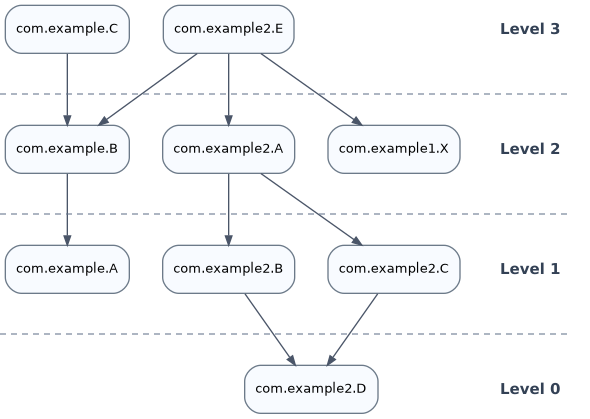
\includegraphics[width=0.75\textwidth]{figures/test-example-classgraph-acyclic-levels.png}
  \caption{Azyklisches Beispiel aus \texttt{test-example-1.0.0.jar}.}
  \label{fig:acyclic-levels}
\end{figure}

Die Pfeile zwischen den Boxen sind Abh\"angigkeiten von Klassen durch Aufruf
oder Nutzung. Im Beispiel nutzt \texttt{com.example.B} die Klasse
\texttt{com.example.A}, kurz $B \to A$. Die horizontalen Linien sind manuell
erg\"anzt und visualisieren die Ebenen der Schichtung. Level~0 bildet das
Fundament; h\"ohere Levels stehen f\"ur Elemente, die von darunterliegenden
Elementen abh\"angen.

Diese Art der Darstellung ist n\"utzlich und weit verbreitet. Als Visualisierung
realer Anwendungen hat sie aber drei praktische Probleme:

\begin{enumerate}
  \item Viele Pfeile machen die Grafik schon bei mittelgro\ss{}en Anwendungen
        un\"ubersichtlich.
  \item Die Paketstruktur ist \"uber mehrere Levels verteilt und bildet keine
        sichtbare Gruppierung.
  \item Bei zyklischen Abh\"angigkeiten muss der Zyklus f\"ur die
        Levelberechnung aufgebrochen werden, damit \"uberhaupt eine vertikale
        Ordnung entsteht. Der urspr\"ungliche Abh\"angigkeitsgraph bleibt
        unver\"andert; ver\"andert wird nur der daraus abgeleitete DAG
        (\emph{Directed Acyclic Graph}, ein gerichteter Graph ohne Zyklen), auf
        dem die Levels berechnet werden. Entscheidend ist deshalb, welche
        Kante f\"ur diese Berechnung ausgeklammert wird, denn genau diese
        Kante erscheint sp\"ater als Bruch der berechneten Ordnung.
\end{enumerate}

\section{S202 als hierarchische Schichtendarstellung}

Mit dem Open-Source-Werkzeug S202 versuchen wir, diese Probleme gezielt zu
adressieren. S202 ersetzt den flachen Klassengraphen nicht einfach durch eine
verbesserte Darstellung, sondern durch eine hierarchische
Architekturhypothese: Pakete bleiben als Container sichtbar, und innerhalb
jedes Containers werden Pakete oder Klassen nach ihren Abh\"angigkeiten
angeordnet.

Die Pfeile k\"onnen optional eingeblendet werden. Im Normalfall soll die
vertikale Ordnung aber bereits ohne Pfeile verst\"andlich machen, welche
Teile der Anwendung weiter oben liegen und welche als Fundament dienen.
Unerw\"unschte Abh\"angigkeiten fallen dadurch nicht als einzelne Linie in einem
gro\ss{}en Netz auf, sondern als Bruch in einer erwarteten Schichtenordnung.

Im Gegensatz zum flachen Klassengraphen sind die Levels bei S202 hierarchisch
durch die Paketstruktur gegliedert. Jedes Paket ordnet seine direkten Kinder,
also Subpakete oder Klassen, nach deren lokalen Abh\"angigkeiten. Die
Paketstruktur bleibt dadurch sichtbar, statt im Klassengraphen
auseinandergezogen zu werden.

\begin{figure}[H]
  \centering
  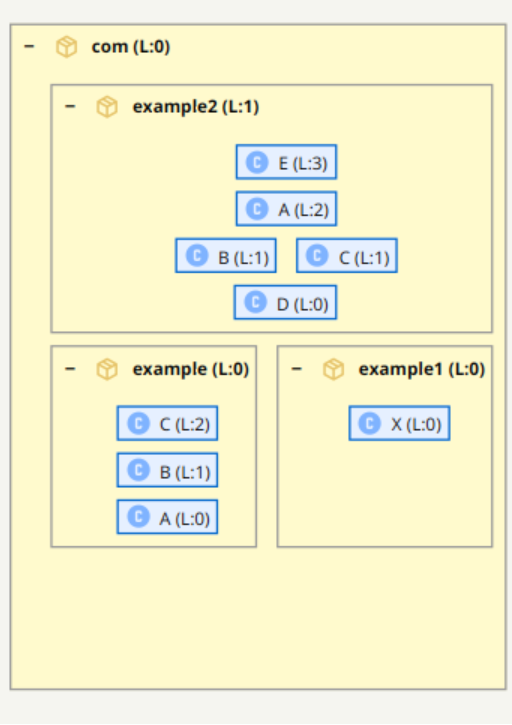
\includegraphics[width=0.55\textwidth]{figures/s202-dependencies-acyclic.png}
  \caption{S202-Darstellung des azyklischen Beispielausschnitts: Pakete
  bleiben als Container sichtbar, Klassen werden innerhalb ihres Containers
  geordnet, und Pfeile k\"onnen bei Bedarf eingeblendet werden.}
  \label{fig:s202-acyclic}
\end{figure}

Das Beispiel zeigt die Paketstruktur unterhalb des \"au\ss{}eren Pakets
\texttt{com}: \texttt{example}, \texttt{example1} und \texttt{example2} sind
Teilb\"aume dieses Containers. Im Teilbaum \texttt{example2} gibt es eine
nicht triviale innere Klassenstruktur; zugleich zeigt die \"ubergreifende Struktur, dass
\texttt{example2} von \texttt{example} und \texttt{example1} abh\"angt. Auf
Klassenebene gilt f\"ur \texttt{example2}: $E \to A \to (B \mid C) \to D$.
Die Darstellung abstrahiert dabei bewusst von einzelnen Kanten. Ob \texttt{A}
eine Abh\"angigkeit nach \texttt{B}, nach \texttt{C} oder nach beiden hat, ist
f\"ur die grobe Architekturansicht weniger wichtig als die Schichtung des
Pakets. Genau diese Abstraktion macht umfangreiche Beziehungsnetze noch lesbar.

Die Idee ist nicht neu. Das kommerzielle Produkt Structure101 hatte bereits
eine sehr \"ahnliche Darstellung. Es gibt jedoch keine offene Implementierung
und keine technische Dokumentation, die erkl\"art, wie man ein solches Layout
zuverl\"assig berechnet. S202 schlie\ss{}t diese L\"ucke als Open-Source-Werkzeug
unter der Apache-Lizenz.

Dieses Dokument beschreibt die typischen Fallstricke bei der Realisierung
eines solchen Layouts und zeigt eine L\"osung, mit der sich viele dieser
Probleme konzeptionell sauber eliminieren lassen.

\section{Typische Fehler bei der Berechnung von Schichten}

Die Abbildungen~\ref{fig:acyclic-levels} und~\ref{fig:s202-acyclic} zeigen
bewusst ein einfaches, azyklisches Beispiel. F\"ur diesen Fall ist die
Schichtung eindeutig: \texttt{E} steht \"uber \texttt{A}, \texttt{A} steht
\"uber \texttt{B} und \texttt{C}, und beide stehen \"uber \texttt{D}. Es gibt
keine R\"uckkopplung, deshalb muss keine Kante ausgew\"ahlt werden, die f\"ur
die Levelberechnung ignoriert wird.

In realen Anwendungen ist dieser Fall eher die Ausnahme. Sobald Klassen oder
Pakete zyklisch voneinander abh\"angen, reicht ein normaler Durchlauf \"uber
den Graphen nicht mehr aus. Genau dort beginnen die interessanten Fehler: Die
Darstellung sieht oft noch plausibel aus, aber die berechneten Ebenen sind
nicht mehr stabil oder nicht mehr fachlich erkl\"arbar.

In den folgenden Abschnitten spielt der Begriff SCC eine zentrale Rolle. Eine
SCC (\emph{Strongly Connected Component}, stark zusammenh\"angende Komponente)
ist eine Menge von Knoten, in der jeder Knoten jeden anderen
\"uber gerichtete Abh\"angigkeitspfade erreichen kann. In einem solchen Zyklus
k\"onnen nicht alle Abh\"angigkeiten gleichzeitig nach unten laufen.

Ein korrektes Schichtlayout muss deshalb gleichzeitig mehrere Anforderungen
erf\"ullen:

\begin{enumerate}
  \item Wenn $A \to B$ gilt, muss $A$ oberhalb von $B$ stehen.
  \item Pakete m\"ussen als Container sichtbar bleiben. Ein Paket darf nicht
        zuf\"allig verschoben werden, nur weil eine einzelne enthaltene Klasse
        ein hohes Klassenlevel hat.
  \item Klassen oder Pakete, die eine SCC bilden, m\"ussen explizit behandelt
        werden, weil in einem Zyklus nicht alle Kanten gleichzeitig nach unten
        laufen k\"onnen.
\end{enumerate}

Diese Anforderungen sind einzeln gut l\"osbar. Zusammen erzeugen sie aber ein
zirkul\"ares Abh\"angigkeitssystem zwischen den Ebenen der Berechnung selbst:
Klassenlevel beeinflussen sichtbare Positionen, Paketcontainer strukturieren
diese Positionen, und SCCs erzwingen Korrekturen an einer Ordnung, die man
ohne Zyklusbehandlung schon berechnet h\"atte. Genau daraus entstehen die
typischen Fehlermodi.

\subsection{Retroaktive Korrektur}

Retroaktive Korrektur bedeutet hier: Eine sp\"ater erkannte Struktur erzwingt
eine nachtr\"agliche \"Anderung an bereits berechneten Levels.

Ein naiver Algorithmus l\"auft \"uber die Klassen und vergibt direkt Level. Er
sieht zuerst Klasse \texttt{A}, setzt ihr Level und hebt damit auch das Paket
von \texttt{A} an. Sp\"ater findet er Klasse \texttt{B} und erkennt: \texttt{A}
und \texttt{B} geh\"oren zu derselben SCC und m\"ussen gemeinsam behandelt
werden. Jetzt m\"usste \texttt{A} korrigiert werden, und damit auch ihr Paket
und m\"oglicherweise weitere Pakete, die davon abh\"angen.

Das Problem ist nicht die Korrektur selbst. Das Problem ist, dass Teile des
Layouts zu diesem Zeitpunkt bereits als fertig behandelt wurden. Ein
Algorithmus, der Zyklenerkennung und Levelvergabe vermischt, muss r\"uckwirkend
an Stellen \"andern, die er eigentlich schon verlassen hat.

\subsection{Reihenfolgeabh\"angige Ergebnisse}

Klassen kommen aus Jars. Die Reihenfolge, in der ein Tool Klassen sieht, folgt
nicht der Architektur, sondern der Packreihenfolge des Jars, der Modulreihenfolge,
dem Build-Tool oder Details des Dateisystems. Wenn ein Algorithmus Zyklen
w\"ahrend dieser Traversierung nebenbei behandelt, h\"angt das Ergebnis von
dieser zuf\"alligen Reihenfolge ab.

Das ist gef\"ahrlich, weil der Fehler nicht sofort sichtbar sein muss. Die
Grafik kann weiterhin ungef\"ahr richtig aussehen. Trotzdem kann dieselbe
Codebasis je nach Build-Konfiguration andere Level bekommen.

\subsection{Vermischte Klassen- und Paketlevel}

Ein naheliegender Fehler ist, das Level eines Pakets aus dem h\"ochsten Level
seiner enthaltenen Klassen abzuleiten. Das klingt plausibel, vermischt aber
zwei verschiedene Fragen: Wo liegt eine Klasse im Klassengraphen, und wo liegt
ein Paket in der Architekturhypothese?

Ein Paket ist nicht deshalb architektonisch hoch, weil es zuf\"allig eine hoch
eingeordnete Klasse enth\"alt. Die zentrale Regel lautet:

\begin{quote}
  Paketlevel entstehen aus Paketabh\"angigkeiten, nicht aus der maximalen
  H\"ohe einzelner Klassen.
\end{quote}

Das klingt trivial, ist es aber nicht. Gerade weil Pakete Container f\"ur
Klassen sind, liegt es nahe, ihre Position aus den enthaltenen Klassen
abzuleiten. Genau dadurch vermischt man jedoch zwei Ebenen, die getrennt
bleiben m\"ussen. Erst wenn Paketlevel aus Paketabh\"angigkeiten entstehen,
bleiben Pakete stabile architektonische Einheiten. Sonst gen\"ugt eine einzige
Ausrei\ss{}er-Klasse, um das Paket auf die falsche Ebene zu heben~-- und damit
den Container unbrauchbar zu machen, der eigentlich Orientierung bieten soll.

\subsection{Der gro\ss{}e See}

Die formal saubere Antwort auf Zyklen lautet: Alle Elemente einer SCC bekommen
dasselbe Level. F\"ur kleine Zyklen ist das akzeptabel. In realen Systemen
k\"onnen SCCs aber sehr gro\ss{} werden. Dann landen Hunderte oder Tausende von
Klassen auf derselben Ebene. Die Schichtung verschwindet; \"ubrig bleibt ein
flacher Block.

Damit wird der Zyklus zwar korrekt erkannt, aber nicht mehr brauchbar
visualisiert. Ein Werkzeug muss gro\ss{}e SCCs daher aufbrechen k\"onnen.
Entscheidend ist, dass die geschnittenen Kanten nicht verschwinden. Sie m\"ussen
sichtbar bleiben, weil genau sie erkl\"aren, warum die berechnete Ordnung nur
als Architekturhypothese gilt.

\section{Der Paketgraph als Architekturhypothese}

Die von S202 gew\"ahlte L\"osung besteht darin, Analyse, Ordnungsbildung und
Darstellung konsequent zu trennen. Der Klassengraph bleibt das Rohmodell der tats\"achlichen
Abh\"angigkeiten. Er wird nicht ver\"andert, nur weil f\"ur eine
Schichtendarstellung ein DAG ben\"otigt wird. Stattdessen erzeugt S202 aus
diesem Graphen zus\"atzliche Sichten: SCCs f\"ur die Zyklenerkennung, einen
gewichteten Paketgraphen f\"ur die Architekturhypothese und eine hierarchische
UI-Struktur f\"ur die Darstellung.

Mit Architekturhypothese ist dabei keine behauptete Soll-Architektur gemeint.
Gemeint ist eine aus den beobachteten Abh\"angigkeiten abgeleitete
Ist-Architektur: die Ordnung, die dem vorhandenen Code und seinen Abh\"angigkeiten
am engsten entspricht, ohne zu verbergen, wo diese Ordnung durch Zyklen oder
R\"uckkanten gebrochen wird.

Die Paketordnung bildet dabei das zentrale Bindeglied. Sie wird nicht aus den
h\"ochsten Klassenlevels abgeleitet, sondern aus den aggregierten
Paketabh\"angigkeiten. Diese Trennung ist der entscheidende Schritt: Klassen
werden innerhalb ihrer Pakete geordnet, Pakete dagegen nach ihren eigenen
Paketbeziehungen. Dadurch kann ein Paket als Container stabil bleiben, auch
wenn einzelne Klassen darin hoch oder niedrig liegen. Gleichzeitig liefert die
Paketordnung ein Kriterium, um Back-Edges nicht beliebig auszuw\"ahlen, sondern
als konkrete Verletzungen der erwarteten Ordnung zu kennzeichnen.

Damit verschwinden die oben beschriebenen Fehlermodi nicht durch einen einzelnen
Algorithmustrick, sondern durch eine klare Zust\"andigkeit der
Berechnungsschritte: Erst werden Abh\"angigkeiten analysiert, dann wird eine
plausible Ordnung bestimmt, danach wird die sichtbare Struktur aufgebaut, und
zuletzt wird gepr\"uft, ob die Darstellung ihre eigene Aussage einh\"alt.

\section{Von Klassenabh\"angigkeiten zur Paketordnung}

Der flache Klassengraph ist in S202 nicht das sichtbare Layoutmodell. Er ist
ein Analyseartefakt: Er dient dazu, konkrete Abh\"angigkeiten zu erfassen, SCCs
zu erkennen, Klassenabh\"angigkeiten zu Paketbeziehungen zu aggregieren und
daraus die sp\"ateren Levels abzuleiten. Die sichtbare S202-Grafik entsteht
danach aus der Paketstruktur und der lokalen Ordnung innerhalb der
Paketcontainer.

Die Paketordnung entsteht lokal im Kontext eines Parent-Pakets. S202
vergleicht nicht beliebige Pakete global miteinander, sondern jeweils die
direkten Kindpakete desselben Containers. Klassen sind in diesem Schritt keine
eigenen Vergleichsknoten. Sie liefern die Information f\"ur die Aggregation:
Eine Klassenabh\"angigkeit wird auf die Kindpakete hochgerollt, in deren
Teilb\"aumen Quelle und Ziel liegen.

F\"ur jedes Parent-Paket entsteht so ein gewichteter Geschwistergraph seiner
Kindpakete. Die Kanten in diesem Graphen sind direkt beobachtete
Paketabh\"angigkeiten zwischen diesen Kindpaketen. Wenn eine Klasse im Teilbaum
von Kindpaket $P$ eine Klasse im Teilbaum von Kindpaket $Q$ benutzt, entsteht
eine Kante $P \to Q$. Ihr Gewicht ist die Anzahl der konkreten Nutzungen, die
auf diese Paketkante hochgerollt werden; f\"ur strukturelle Abh\"angigkeiten
ohne Aufrufz\"ahlung wird ein Gewicht von~1 verwendet. Die Gegenrichtung wird
ebenfalls gez\"ahlt.

Der Geschwistergraph enth\"alt nur solche direkten Paketabh\"angigkeiten. Aus
$B \to A$ und $C \to B$ wird keine zus\"atzliche Kante $C \to A$ erzeugt. Die
transitive Ordnung entsteht erst bei der anschlie\ss{}enden Levelberechnung.
Abh\"angigkeiten innerhalb desselben Kindpakets ver\"andern die Ordnung der
Kindpakete nicht; Abh\"angigkeiten, die den Parent-Container verlassen, werden
auf einer h\"oheren Ebene der Paketstruktur behandelt. Dieser Vergleich wird
rekursiv f\"ur alle Paketcontainer wiederholt. Die Ordnung der Klassen
innerhalb eines Paketcontainers ist ein nachgelagerter Schritt.

Vor der Levelberechnung muss der Geschwistergraph azyklisch sein. Bilden
Kindpakete eine SCC, bewertet S202 mit einem Rangma\ss{}, ob ein Kindpaket im
aktuellen Geschwistergraphen eher andere Pakete nutzt oder eher von ihnen
genutzt wird:

\[
  rank(P) = \frac{out(P) - in(P)}{\max(1,\; out(P) + in(P))}
\]

$out(P)$ ist die Summe der Kantengewichte von $P$ zu anderen betrachteten
Geschwistern im aktuellen Graphen, $in(P)$ die Summe der Kantengewichte aus
diesen Geschwistern nach $P$. Ein positiver Rang bedeutet: Das Paket
benutzt mehr, als es selbst benutzt wird; es geh\"ort tendenziell nach oben.
Ein negativer Rang bedeutet: Das Paket wird eher benutzt und geh\"ort
tendenziell nach unten.

In einer Paket-SCC wird eine Kante $P \to Q$ erst dann als Back-Edge behandelt,
wenn $rank(P)$ um mehr als eine Schwelle $\varepsilon$ unter $rank(Q)$ liegt.
In S202 wird daf\"ur aktuell $\varepsilon = 0{,}1$ verwendet. Liegen zwei
Pakete zu nah beieinander, bleiben sie konzeptionell Peers und damit auf
demselben Level. Ein gegenseitiges Aufrufverh\"altnis von $100 : 101$ ist
deshalb keine belastbare Architekturentscheidung.

Nach dieser Zyklusbehandlung berechnet S202 die Levels auf dem resultierenden
DAG. Level~0 bilden die Pakete, die im aktuellen Berechnungsgraphen keine
weiteren Kindpakete benutzen. Jedes andere Paket liegt eine Ebene \"uber dem
h\"ochsten Kindpaket, das es direkt benutzt. Dadurch entsteht die transitive
Schichtung: Aus $B \to A$ und $C \to B$ folgt $A$ auf Level~0, $B$ auf
Level~1 und $C$ auf Level~2, auch wenn keine direkte Kante $C \to A$ existiert.

\section{Vom Klassenzyklus zur Paketordnung}

Abbildung~\ref{fig:cyclic-class} zeigt ein zyklisches Beispiel aus dem
Example-Jar als klassischen Klassengraphen. Die beiden Teilgraphen f\"ur Notification und
Payment enthalten jeweils R\"uckkopplungen.

\begin{figure}[H]
  \centering
  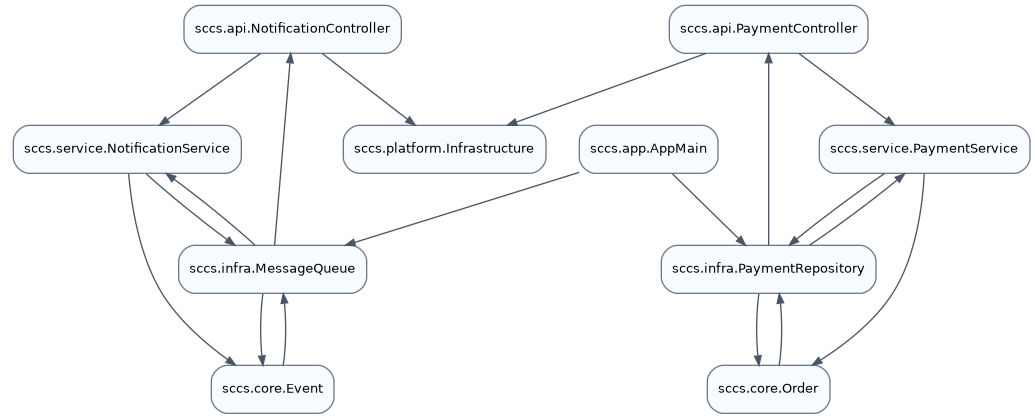
\includegraphics[width=0.9\textwidth]{figures/test-example-classgraph-cyclic.png}
  \caption{Zyklisches Beispiel aus \texttt{test-example-1.0.0.jar}. In jedem
  Zyklus muss mindestens eine Kante f\"ur die Levelberechnung geschnitten werden.}
  \label{fig:cyclic-class}
\end{figure}

Die markierten zyklischen Bereiche sind zwei nicht-triviale SCCs: eine
Notification-SCC mit \texttt{NotificationController}, \texttt{NotificationService},
\texttt{MessageQueue} und \texttt{Event}, sowie eine Payment-SCC mit
\texttt{PaymentController}, \texttt{PaymentService}, \texttt{PaymentRepository}
und \texttt{Order}. Das etablierte Verfahren zur Ermittlung solcher Komponenten
ist der Tarjan-Algorithmus.

Damit stellt der Klassengraph im Zyklusfall die technische Frage: Welche Kante
muss man ignorieren, damit aus der SCC wieder ein berechenbarer DAG f\"ur die
Levelbildung wird? Der Klassengraph allein liefert daf\"ur aber kein fachliches
Kriterium. Erst die Paketordnung liefert dieses Kriterium: Eine als Back-Edge
klassifizierte Kante ist dann keine beliebige Schnittkante im flachen
Klassengraphen, sondern eine konkrete Abh\"angigkeit, die gegen die berechnete
Paketordnung l\"auft und damit den Bruch in der Architekturhypothese sichtbar
macht.

\begin{figure}[H]
  \centering
  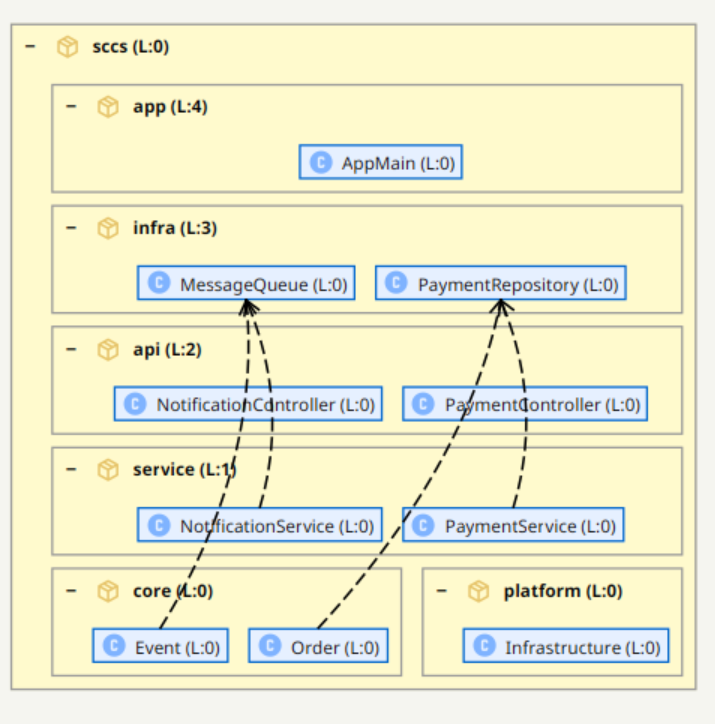
\includegraphics[width=0.6\textwidth]{figures/s202-dependencies-cyclic.png}
  \caption{Zyklisches Beispiel in der S202-Darstellung. Die gestrichelten Kanten sind Verletzungen:
  Sie laufen gegen die aus den Paketabh\"angigkeiten abgeleitete Ordnung und
  bleiben als sichtbarer Befund der Architekturhypothese erhalten. Alle vier
  gestrichelten Kanten geh\"oren zu den zwei SCCs und werden von S202 als
  Back-Edges f\"ur die Levelberechnung klassifiziert.}
  \label{fig:s202-cyclic}
\end{figure}

Die Begriffe Back-Edge und Verletzung beschreiben unterschiedliche Rollen:

\begin{description}
  \item[Back-Edge] Eine ausgew\"ahlte Kante innerhalb einer SCC, die f\"ur die
        Levelberechnung gesondert behandelt wird, damit der Berechnungsgraph
        azyklisch wird. Sie geh\"ort zur Zyklusbehandlung.
  \item[Verletzung] Eine konkrete Abh\"angigkeit, die nach der berechneten
        Ordnung nach oben l\"auft. Sie kann aus einer SCC stammen, muss es aber
        nicht. Verletzungen sind damit eine Obermenge der Back-Edges: Eine
        Back-Edge kann als Verletzung sichtbar werden, aber nicht jede
        Verletzung ist eine Back-Edge. Begrifflich bleibt eine Verletzung die
        sichtbare Ordnungsabweichung, w\"ahrend eine Back-Edge die Rolle der
        Kante in der Zyklusbehandlung beschreibt.
\end{description}

S202 versteckt den Zyklus daher nicht. Als Back-Edges klassifizierte Kanten
bleiben als Verletzungen sichtbar, weil sie erkl\"aren, warum die Paketordnung
nicht vollst\"andig zu den konkreten Klassenabh\"angigkeiten passt. Dadurch wird
die Abweichung nachvollziehbar statt beliebig.

\section{Redundante Pr\"ufung der Konsistenz}

Die bisher beschriebenen Schritte zeigen bereits, warum die Umsetzung
fehleranf\"allig ist. Es reicht nicht, einzelne Algorithmen isoliert mit Unit
Tests abzusichern. Viele Fehler entstehen erst durch das Zusammenspiel der
Daten: konkrete Klassenabh\"angigkeiten, Paketstruktur, SCCs, aggregierte
Paketgewichte und lokale Darstellungspositionen beeinflussen sich gegenseitig.

S202 pr\"uft deshalb nicht nur einzelne Rechenschritte. Nachdem die komplette
Pipeline gelaufen ist, wird das fertige Ergebnis redundant gegen
Konsistenzregeln gepr\"uft. Diese Regeln berechnen das Layout nicht neu und
korrigieren auch nichts. Sie lesen nur das Ergebnis und fragen: Ist die
erzeugte Darstellung in sich stimmig?

Die Pr\"ufung betrachtet drei Ebenen:

\begin{enumerate}
  \item \textbf{Klassengraph:} F\"ur normale Klassenabh\"angigkeiten muss
        gelten: Wenn $A \to B$, dann steht $A$ auf einem h\"oheren Level als
        $B$. Ausnahmen m\"ussen explizit klassifiziert sein, zum Beispiel als
        Back-Edge oder als Kante innerhalb einer SCC.
  \item \textbf{Paketgraph:} Die berechnete Paketordnung muss zu den
        gewichteten Paketabh\"angigkeiten passen. Pakete mit h\"oherem Rang
        m\"ussen oberhalb der Pakete liegen, von denen sie st\"arker abh\"angen.
        Kanten, die beim Aufbrechen einer Paket-SCC geschnitten werden, d\"urfen
        in dieser Pr\"ufung nicht wie normale dominante Kanten behandelt werden;
        sie m\"ussen gesondert als Paket-Back-Edges klassifiziert sein.
  \item \textbf{Sichtbare Darstellung:} Die sichtbare Anordnung muss zum berechneten
        Modell passen. Paketcontainer, lokale Klassenpositionen und
        verschachtelte Levels d\"urfen die berechnete Architekturhypothese nicht
        stillschweigend umkehren.
\end{enumerate}

Diese Konsistenzregeln sind keine zus\"atzliche Optimierung und kein zweiter
Layoutalgorithmus. Sie sind ein unabh\"angiger Plausibilit\"atscheck nach
Abschluss der Berechnung. Genau dadurch finden sie Fehler, die in normalen
Unit Tests leicht fehlen: ein Paketlevel wurde korrekt berechnet, aber lokal
falsch dargestellt; eine Back-Edge wurde geschnitten, aber nicht als solche
markiert; eine normale Kante l\"auft nach oben, ohne dass sie Teil einer SCC ist.

Der entscheidende Punkt ist Redundanz. Die Pipeline erzeugt die Darstellung.
Die Regeln pr\"ufen anschlie\ss{}end, ob diese Darstellung ihre eigene Aussage
einh\"alt. Damit wird aus einer reinen Grafik ein \"uberpr\"ufbares Modell.

\section{Von der Visualisierung zur Aktion}

Eine berechnete Architekturhypothese ist besonders dann n\"utzlich, wenn sie
nicht nur einen Zustand beschreibt, sondern Ver\"anderung planbar macht. S202
enth\"alt daf\"ur eine What-If-Analyse: Klassen und Pakete k\"onnen per Drag
and Drop in der Darstellung verschoben werden. Das Modell wird dadurch nicht
sofort refaktoriert; stattdessen berechnet das Werkzeug, welche Abh\"angigkeiten
in der neuen Anordnung nach oben laufen w\"urden.

Die Verletzungen aktualisieren sich nach jeder Verschiebung. Dadurch wird
sichtbar, ob eine geplante Umordnung die Architektur konsistenter macht oder
neue Probleme erzeugt. Das ist vor allem in Situationen wichtig, in denen das
Werkzeug keine eindeutige Ordnung mehr findet: gro\ss{}e SCCs, symmetrische
Paketabh\"angigkeiten oder historisch gewachsene Kopplungen lassen sich nicht
immer automatisch sinnvoll aufl\"osen.

\begin{figure}[H]
  \centering
  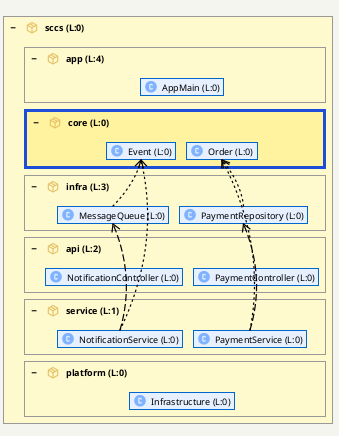
\includegraphics[width=0.45\textwidth]{figures/whatif-core-over-infra.png}
  \caption{What-If-Verschiebung: Das Paket \texttt{core} wird aus Level~0
  zwischen Level~3 und Level~4 verschoben. Dadurch entstehen sechs
  Verletzungen, weil bestehende Abh\"angigkeiten nun gegen die gew\"ahlte
  Anordnung laufen.}
  \label{fig:whatif-core-over-infra}
\end{figure}

Abbildung~\ref{fig:whatif-core-over-infra} zeigt genau diese Arbeitsweise:
Die manuelle Anordnung entspricht nicht mehr der aus den Abh\"angigkeiten
berechneten Ordnung. Sie kann trotzdem eine gew\"unschte Zielarchitektur
ausdr\"ucken, etwa wenn \texttt{core} fachlich oberhalb der Infrastruktur
liegen soll. S202 behandelt diese Entscheidung deshalb nicht als Fehler der
Darstellung, sondern macht ihre Kosten sichtbar: In diesem Fall m\"ussten sechs
konkrete Beziehungen refaktoriert oder entkoppelt werden, damit die
Abh\"angigkeiten wieder zur gew\"ahlten Schichtung passen.

Erg\"anzend dazu gibt es eine manuelle CUT-Logik. Back-Edges k\"onnen gezielt
als geplante Schnitte markiert werden, und das Werkzeug kann anschlie\ss{}end
pr\"ufen, ob diese Schnitte die betroffene SCC tats\"achlich aufl\"osen. Der
Benutzer sieht nicht nur, welche Kante als Bruch der Ordnung plausibel w\"are,
sondern kann die Wirkung dieses Schnitts auf den Zyklus \"uberpr\"ufen.

Diese CUT-Logik arbeitet feiner als die sichtbare Klassen- oder Paketkante.
Geschnitten wird auf Methodenaufrufebene: Nicht zwingend die gesamte Beziehung
zwischen zwei Klassen verschwindet, sondern der konkrete Methodenaufruf, der
die zyklische Abh\"angigkeit verursacht. Dadurch passt das Feature besser zur
praktischen Refactoring-Arbeit, weil ein Zyklus oft durch wenige konkrete
Aufrufe entsteht, nicht durch die komplette fachliche Beziehung zweier Klassen.

\section{Umsetzung auf konzeptioneller Ebene}

Die Umsetzung trennt die Berechnung bewusst in mehrere Phasen. Entscheidend
ist, dass keine Phase eine sichtbare Position festlegt, bevor die Informationen
vorliegen, die diese Position begr\"unden.

\begin{enumerate}
  \item \textbf{Klassengraph aufbauen:} Aus dem Bytecode wird ein gerichteter
        Klassengraph erzeugt. Dieser Graph bleibt das fachliche Rohmodell der
        Analyse.
  \item \textbf{SCCs erkennen:} Auf dem Klassengraphen werden stark
        zusammenh\"angende Komponenten mittels Tarjan ermittelt. Das Ergebnis
        ist noch kein Layout, sondern die Information, welche Klassen azyklisch
        einordenbar sind und welche zu Zyklen geh\"oren.
  \item \textbf{Paketgraph ableiten:} Aus den Klassenabh\"angigkeiten werden
        Paketabh\"angigkeiten aggregiert und gewichtet.
  \item \textbf{Paketordnung berechnen:} Aus den gewichteten Ein- und Ausg\"angen
        wird das Rangma\ss{} $rank(P)$ berechnet. Daraus entsteht die vertikale
        Paketordnung. Kleine Rangunterschiede werden als Peer-Beziehung behandelt.
  \item \textbf{Back-Edges bestimmen:} Innerhalb jeder SCC werden die Kanten
        ausgew\"ahlt, die f\"ur die Zyklusentfernung ausreichen. Diese Kanten
        sind Back-Edges f\"ur die Levelberechnung und bleiben zugleich als
        Verletzungen sichtbar, wenn sie nach der berechneten Ordnung nach oben
        laufen.
        \emph{Geschnitten} bedeutet dabei nicht, dass die Kante aus dem Modell
        verschwindet. Sie wird nur f\"ur den DAG der Levelberechnung ausgenommen
        und bleibt als Befund erhalten.
  \item \textbf{Lokale Schichtung aufbauen:} Erst danach wird die sichtbare
        Baumstruktur erzeugt. Innerhalb jedes Containers werden nur die direkten
        Kinder angeordnet. Dadurch wird die globale Paketordnung nicht mit
        lokalen Klassenlevels vermischt.
  \item \textbf{Konsistenz pr\"ufen:} Zum Schluss wird die fertige Darstellung
        redundant gegen die Konsistenzregeln gepr\"uft. Normale Abh\"angigkeiten,
        SCCs, Back-Edges und Verletzungen werden unterschieden und klassifiziert.
\end{enumerate}

Kurz gefasst:

\begin{lstlisting}
Bytecode -> Klassengraph -> SCCs -> Paketgraph -> Paketordnung
         -> Back-Edges -> sichtbare Schichtung -> Konsistenzregeln
\end{lstlisting}

\section{Fazit}

S202 berechnet aus den bestehenden Abh\"angigkeiten die plausibelste Hypothese
der Ist-Architektur. Das Ergebnis ist eine \"uberpr\"ufbare hierarchische
Schichtendarstellung: Klassenabh\"angigkeiten liefern den Graphen,
Paketabh\"angigkeiten liefern eine belastbare Ordnung, Back-Edges machen
notwendige Br\"uche sichtbar, und Konsistenzregeln pr\"ufen, ob die fertige
Darstellung ihre eigene Aussage einh\"alt.

Der wichtigste Beitrag liegt deshalb nicht in einer optisch verbesserten
Grafik, sondern in der Verbindung von Darstellung, Erkl\"arung und
Ver\"anderbarkeit. Die
Schichtung zeigt eine m\"ogliche Ordnung. Die markierten Befunde erkl\"aren,
wo diese Ordnung durch konkrete Abh\"angigkeiten gebrochen wird. What-If-Verschiebungen
und manuelle CUTs machen sichtbar, welche Refactorings diese Br\"uche reduzieren
oder Zyklen tats\"achlich aufl\"osen k\"onnen.

Damit ist die Visualisierung mehr als ein Layout. Sie ist ein erkl\"arbares
Arbeitsmodell: Jede Position und jede hervorgehobene Kante muss auf eine
nachvollziehbare Entscheidung in der Berechnung zur\"uckf\"uhrbar sein, und
jede geplante \"Anderung kann gegen dieselbe Ordnung gepr\"uft werden.

\end{document}
